\theoremstyle{plain}% default
\newtcbtheorem[number within=section]{definicion}%
 {\textsc{Definici\'on}}{theorem style=plain, sharp
corners,enhanced,colframe=blue!50!black,colback=yellow!20!white,coltitle=red!50!black,fonttitle=\upshape\bfseries\large,fontupper=\itshape,
drop lifted shadow=blue!70!black!50!white,boxrule=0.4pt}{definicion}
%
%
%fontupper=\itshape\large
%
\newtcbtheorem[use counter from=definicion]{teorema}%
 {\textsc{Teorema}}{theorem style=plain,sharp
corners, enhanced,colframe=blue!50!black,colback=yellow!20!white,
coltitle=red!50!black,fonttitle=\upshape\bfseries\large,fontupper=\itshape,
drop lifted shadow=blue!70!black!50!white,boxrule=0.4pt}{teorema}
%
%
%
%
\newtcbtheorem[use counter from=definicion]{lema}%
  {\textsc{Lema}}{theorem style=plain, sharp
corners,enhanced,colframe=blue!50!black,colback=yellow!20!white,
coltitle=red!50!black,fonttitle=\upshape\bfseries\large,fontupper=\itshape,drop lifted shadow=blue!70!black!50!white,boxrule=0.4pt}{lema}
%
%
%
%
\newtcbtheorem[use counter from=definicion]{corolario}%
  {\textsc{Colorario}}{theorem style=plain,sharp
corners, enhanced,colframe=blue!50!black,colback=yellow!20!white,
coltitle=red!50!black,fonttitle=\upshape\bfseries\large,fontupper=\itshape,
drop lifted shadow=blue!70!black!50!white,boxrule=0.4pt}{colorario}
%
%
%
%
%
\newtcbtheorem[use counter from=definicion]{proposicion}%
  {\textsc{Proposici\'on}}{theorem style=plain,sharp
corners, enhanced,colframe=blue!50!black,colback=yellow!20!white,
coltitle=red!50!black,fonttitle=\upshape\bfseries\large,fontupper=\itshape,
drop lifted shadow=blue!70!black!50!white,boxrule=0.4pt}{proposicion}
%
%
%
\newtcbtheorem[number within=chapter]
{observacion}%
{\textsc{Observaci\'on}}{theorem style=plain,sharp
corners, enhanced,colframe=blue!50!black,colback=blue!5!white,
coltitle=red!50!black,fonttitle=\upshape\bfseries\normalsize,fontupper=\itshape,
drop lifted shadow=blue!70!black!50!white,boxrule=0.6pt}{observacion}
%
%
 % 
\newtcbtheorem[auto counter,number within=section]{notacion}%
  {\textsc{Notaci\'on}}{fonttitle=\bfseries\upshape\large, fontupper=\slshape,
     arc=0mm, colback=blue!0!white,colframe=blue!0!white}{notacion}
%
%
%
\theoremstyle{definition}
\newtheorem{Ejemplo}{Ejemplo}[section]
%---------------------------------------------------------------
%{\begin{pspicture}(0.62,0)(2.6,0.4)
%\psline[linecolor=red!50!black, linewidth=1pt](0.6,-0.1)(3.8,-0.1)
%\psline[linecolor=red!50!black, linewidth=1pt](0.6,-0.1)(0.6,0.4)
%\rput(1.7,0.1){{\large\textsc{Ejemplo}}}
%\end{pspicture}}
%
%------------------------------------------------------------------------------
%%%%%%%%%%%%%%%%%% new style teorem %%%%%%%%%%%%%%%%%%%%%%%
\newtheoremstyle{ejer}  % name of the style to be used
   {10mm}       % measure of space to leave above the theorem. E.g.: 3pt
   {10mm}       % measure of space to leave below the theorem. E.g.: 3pt
   {\slshape}   % name of font to use in the body of the theorem
   {6pt}        % measure of space to indent
   {\bfseries}  % name of head font
   {\newline}   % punctuation between head and body
   {10pt}       % space after theorem head
   {\fcolorbox{red!50!black}{white}{Ejercicio.\thmnumber{ #2}}}           % Manually specify head
\theoremstyle{ejer}
\newtheorem{ejer}{Ejercicio:}
%%%%%%%%%%%%%%%%%%%%%%%%%%%% cambio de margen %%%%%%%%%%%%%%%%%%%%%%%%%%%%%%%%%
\newenvironment{cmargen}[1]{\begin{minipage}[c]{#1\linewidth}}{\end{minipage}}
%%%%%%%%%%%%%%%%%%%%%%%%%%%%%%%%%%%%%%%%%%%%%%%%%%%%%%%%%%%%%%%%%%%%%%%%%%%%%%%
%\theoremstyle{plain}
%\newtheorem{ejer}{Ejercicios
%\begin{pspicture}(0,0)(0,0)
%%\psgrid
%\psline[linecolor=red!50!black, linewidth=1pt](-2.1,-0.2)(1.5,-0.2)
%\psline[linecolor=red!50!black, linewidth=1pt](-2.1,-0.2)(-2.1,0.5)
%\psline[linecolor=red!50!black, linewidth=1pt](1.5,-0.2)(1.5,0.5)
%\psline[linecolor=red!50!black, linewidth=1pt](-2.1,0.5)(1.5,0.5)
%\end{pspicture}
%}[section]

%\hspace{-0.67cm}
%
\newcommand{\solucion}{ \textcolor{red!50!black}{ \textsc{\bf Soluci\'on: }}}
%
%\newcommand{\acc}[1]{
%{\begin{pspicture}(0,0)(2.5,0.5)
%%\psgrid
%%\psline[linecolor=Turquoise, linewidth=2pt](0,0)(2.5,0)
%%\psline[linecolor=Turquoise, linewidth=2pt](0,0)(0,0.5)
%\rput(1.5,0.2){\Large \textcolor{MidnightBlue}{Actividad #1}}
%\end{pspicture}}}
%
\newcommand{\acc}[1]{\fcolorbox{MidnightBlue}{white}{\bfseries{Actividad}:\ #1}} 
%
\def\QEDmark{\ensuremath{\square}}
%
\def\proof{\paragraph{\textcolor{red!50!black}{ \textsc{\bf Soluci\'on.}}}}
\def\endproof{\hfill\color{red!50!black}$\blacksquare$}
%
%%%%%%%%%%%%%%%%%%%%%%%%%%%%% para la demostración %%%%%%%%%%%%%%%%%%%%%
\newcommand{\demostracion}{ \textcolor{red!50!black}{\hspace{-0.67cm}\textsc{ \bf Demostraci\'{o}n.}\,}}
%
%
%%%%%%%%%%%%%% MALLA %%%%%%%%
  \newpsobject{malla}{psgrid}{subgriddiv=1,griddots=10,gridlabels=6pt}
\allowdisplaybreaks
\setlength{\parindent}{0pt}
%
%
%
%%%%%%%%%%%%%%%%%%%%%%%%%%%%%%%%%%%%%%%%%%%%%%%%%%%%%%%%%%%%%%%%%%%
\newcommand{\Co}{\mathbb C}
\newcommand{\F}{\mathbb F}
\newcommand{\J}{\mathbb J}
\newcommand{\K}{\mathbb K}
\newcommand{\N}{\mathbb N}
\newcommand{\Po}{\mathbb P}
\newcommand{\Q}{\mathbb Q}
\def\R{I\!\! R}
\newcommand{\Z}{\mathbb Z}
\renewcommand{\K}{\mathbb K}
\newcommand{\Rd}{\ensuremath{\R^2}}
\newcommand{\Rt}{\ensuremath{\R^3}}
\newcommand{\Ro}{\ensuremath{\R_0}}
\newcommand{\No}{\ensuremath{\N_0}}
%
%%%%%%%%%%%%%%%%%%%%%%%%%%%%%%%%%%%%%%%%%%%%%%
%FLECHAS
\newcommand{\infinitot}{t\to\infty}  % t tiende hacia infinito
\newcommand{\infiniton}{n\to\infty}  % n tiende hacia infinito
\newcommand{\hacia}{\longrightarrow}
\newcommand{\ssi}{\longleftrightarrow}
\newcommand{\Ssi}{\Longleftrightarrow}
\newcommand{\implica}{\Longrightarrow}
\newcommand{\reciproca}{\longleftarrow}
\newcommand{\xtoa}[2]{#1\to #2}
%%%%%%%%%%%%%%%%%%%%%%%%%%%% límites%%%%%%%%%%%%%%%%%%%%%%%%%%%%%%%%%%%%%%%%%%%
\newcommand{\funcreal}[2]{\ensuremath{\,#1\!:#2\rightarrow \mathbb R\,}}
\newcommand{\cfunc}[2]{\ensuremath{\,#1:#2\rightarrow \mathbb C\,}}
\newcommand{\circulo}{\marginpar{\vspace{0.3cm}\hspace{-16.7cm}$\circledS$}{}}%LIMITES
\newcommand{\nlim}{\lim\limits_{n\to\infty}}
\newcommand{\tlim}{\lim\limits_{t\to\infty}}
\newcommand{\jlim}{\lim\limits_{j\to\infty}}
\newcommand{\klim}{\lim\limits_{k\to\infty}}
\newcommand{\mlim}{\lim\limits_{m\to\infty}}
\newcommand{\rlim}{\lim\limits_{r\to\infty}}
\newcommand{\limin}[1]{\lim\limits_{#1\to +\infty}}
\newcommand{\limmin}[1]{\lim\limits_{#1\to - \infty}}
\newcommand{\Limd}[3]{\mbox{$\displaystyle{\lim_{#2\to #3^+}#1}$}}
\newcommand{\Limi}[3]{\mbox{$\displaystyle{\lim_{#2\to #3^-}#1}$}}
\newcommand{\Lim}[3]{\mbox{$\displaystyle{\lim_{#2\to #3}#1}$}}
\newcommand{\limlft}[3]{\mbox{$\dis{\lim_{\substack{#2\to #3\\ #2\,<\,#3}}#1}$}}
\newcommand{\limrgt}[3]{\mbox{$\dis{\lim_{\substack{#2\to #3\\ #2\,>\,#3}}#1}$}}
\newcommand{\Btag}{\tag*{$\Box$}}
%%%%%%%%%%%%%%%%%%%%%%%%%%%%%%%%%%%%%%%%%%%%%%%%%%%%%%%%%%%%%%%%%%%%%%%%%%%%%%%%
%SUMAS
\newcommand{\Sumai}{\sum\limits_{i=1}^n}     %Suma desde i=1 hasta n (con el \limits)
\newcommand{\sumai}{\sum_{i=1}^n}             %Suma desde i=1 hasta n (sin el \limits)
\newcommand{\Sumaj}{\sum\limits_{j=0}^{n-1}}      %Suma desde j=0 hasta n-1
\newcommand{\Suman}{\sum\limits_{n=1}^\infty}   %Suma desde n=1 hasta  infinito
\newcommand{\suman}{\sum\limits_{n=0}^\infty}   %Suma desde n=0 hasta  infinito
\newcommand{\jSuma}{\sum\limits_{j=1}^\infty}   %Suma desde j=1 hasta  infinito
\newcommand{\jsuma}{\sum_{j=1}^\infty}   %Suma desde j=1 hasta  infinito
\newcommand{\Sumak}{\sum\limits_{k=0}^\infty}     %Suma desde k=0 hasta infinito (con el \limits)
\newcommand{\sumak}{\sum\limits_{k=1}^\infty}     %Suma desde k=1 hasta infinito (con el \limits)
\newcommand{\serie}[1]{\sum\limits_{#1}^\infty} 
\newcommand{\suma}[2]{\sum\limits_{#1}^#2} 
%%%%%%%%%%%%%%%%%%%%%%%%%%%%%%%%%
\newcommand{\dis}{\displaystyle}
%\newcommand{\Int}{\displaystyle\int}
%\newcommand{\rig}{\rightarrow}
%\newcommand{\lef}{\leftarrow}
%\newcommand{\Rig}{\Rightarrow}
%
%%%%%% Funciones trigonometrica e hiperbolicas %%%%%%%%%
\newcommand{\sen}{\operatorname{\sen}}
%\newcommand{\cos}{\operatorname{\cos}}
\newcommand{\arcsec}{\mathop{\rm arcsec}\nolimits}
\newcommand{\arcsen}{\mathop{\rm arcsen}\nolimits}
\newcommand{\arccot}{\mathop{\rm arccot}\nolimits}
\newcommand{\arccsc}{\mathop{\rm arccsc}\nolimits}
\newcommand{\senh}{\mathop{\rm senh}\nolimits}
\newcommand{\secanteh}{\mathop{\rm sech}\nolimits}
\newcommand{\cosecanteh}{\mathop{\rm csch}\nolimits}
%%%%%%%%%%%%%%%%%%%%% derivadas %%%%%%%%%%%%%%%%%%%%%%%%%%%%%%%%%%%%%%%%%%%%%%%
%%%%%%%%%%%%%%%%%%%%%%%%%%%%% DERIVAR  %%%%%%%%%%%%%%%%%%%%%
%\providecommand{\derive}[2]{\frac{d }{ d  #2}\left[#1\right]}
%
%
\providecommand{\deriven}[2]{\dfrac{d^n#1 }{ d  #2^n}}
\providecommand{\derive}[2]{\dfrac{d #1 }{ d  #2}}
\providecommand{\derivee}[2]{\dfrac{d^2#1 }{ d  #2}}
\newcommand{\Dfa}{\mbox{$f^{\,\prime}(a)$}}
\newcommand{\Dfka}{\mbox{$f^{\,(k)}(a)$}}
\newcommand{\Dfna}{\mbox{$f^{\,(n)}(a)$}}
\newcommand{\derivada}[2]{\ensuremath{\dfrac{\mathrm{d} #1}{\mathrm{d}#2}}}  % Derivada de #1 respecto de #2
\newcommand{\derivadados}[2]{\ensuremath{\dfrac{\mathrm{d}^2 #1}{\mathrm{d}#2^2}}}
\newcommand{\derivadatres}[2]{\ensuremath{\dfrac{\mathrm{d}^3 #1}{\mathrm{d}#2^3}}}
\newcommand{\derivadan}[2]{\ensuremath{\dfrac{\mathrm{d}^n #1}{\mathrm{d}#2^n}}}
\newcommand{\fder}[1]{\mbox{$#1^{\,\prime}$}}
\newcommand{\Derdos}[2]{\mbox{$#1^{\,\prime\prime}(#2)$}}
\newcommand{\derpar}[2]{\mbox{$\dfrac{\partial #1}{\partial #2}$}}
\newcommand{\derpardos}[2]{\mbox{$\dfrac{\partial^{2}\! #1}{\partial #2^{2}}$}}
\newcommand{\scd}{\mbox{$^{\,\prime\prime}$}}
\newcommand{\Der}[2]{\mbox{$#1^{\,\prime}(#2)$}}
\newcommand{\Derk}[2]{\mbox{$#1^{\,(k)}(#2)$}}
\newcommand{\Dern}[2]{\mbox{$#1^{\,(n)}(#2)$}}
\newcommand{\partx}[1]{\ensuremath{\dfrac{\partial #1}{\partial x}}}
\newcommand{\party}[1]{\ensuremath{\dfrac{\partial #1}{\partial y}}}
\newcommand{\partz}[1]{\ensuremath{\dfrac{\partial #1}{\partial z}}}
\newcommand{\partxx}[1]{\ensuremath{\dfrac{\partial^2 #1}{\partial x^{2}}}}
\newcommand{\partyy}[1]{\ensuremath{\dfrac{\partial^2 #1}{\partial y^2}}}
\newcommand{\partxy}[1]{\ensuremath{\dfrac{\partial^2 #1}{\partial x
\partial y}}}
\newcommand{\partyx}[1]{\ensuremath{\frac{\partial^2 #1}{\partial y
\partial x}}}
\newcommand{\partone}[2]{\ensuremath{\dfrac{\partial #1}{\partial #2}}}
\newcommand{\partwo}[2]{\ensuremath{\dfrac{\partial^2 #1}{\partial #2^2}}}
\newcommand{\Dpd}[2]{\ensuremath{D_{#2}#1}}
\newcommand{\Dpxy}[3]{\ensuremath{D_{#2 #3}#1}}
\newcommand{\Dp}[3]{\ensuremath{\partial_{#1}#2(#3)}}
\newcommand{\partonetwo}[3]{\ensuremath{\dfrac{\partial^2 #1}{\partial #2\partial #3}}}
%%%%%%%%%%%%%%%%%%%%%%%%%%%%%%%%%%%%%%%%%%%%%%%%%%%%%%%%%%%%%%%%%%%%%%%%%%%%%%%
\newcommand{\derparcial}[2]{\ensuremath{\dfrac{\partial #1}{\partial
#2}}}
%%%%%%%%%%%%%%%%%%%%%%%%%%%%%%%%%%%%%%%%%%%%%%%%%%%%%%%%%%%%%%%%%%%%%%%%%%%%%%%
\renewcommand{\partname}{Semana}
%\newtheorem{proof}{Remark}
%\renewcommand*{\proofname}{Solution}
%
\def\@sqrt[#1]{\root #1\of}
%
%\renewcommand{\rmdefault}{phv}
%\renewcommand{\sfdefault}{phv}
\normalfont
%%%%%%%%%%%%%%%% cajas espciales%%%%%%%%%%%%%%%%%%
%
%%%%%%%%%%%%%%%%%%%% Otros comandos %%%%%%%%%%%%%%%%%%%%%%%%%%%%%%%
%%%%%%%%%%%%%%% ------ colores ---------------%%%%%%%%%%%%%%%%%%%%%
\definecolor{problemblue}{RGB}{100,134,158}
\definecolor{titlebgdark}{RGB}{10,76,115}
\definecolor{ocre}{RGB}{10,76,115}
\definecolor{ptctitle}{RGB}{10,76,115}
\definecolor{ptcbackground}{RGB}{212,237,252}
\definecolor{titlebglight}{RGB}{191,233,251}
%%%%%%%%%%%%%%%%%%%%%%%%%%%%%%%%%%%%%%%%%%%%%%%%%%%%%
\newcommand\peque{\@setfontsize\peque{8}{9}}
\newcommand{\remark}{\colorbox{titlebgdark}{\color{white}{\bfseries Nota:}} }
\newcommand{\prop}{\colorbox{titlebgdark}{\color{white}{\bfseries Proposici\'on:}} }
\newcommand{\dem}{\colorbox{titlebgdark}{\color{white}{\bfseries Demostraci\'on:}} }
\newcommand{\notacionn}{\colorbox{titlebgdark}{\color{white}{\bfseries Notaci\'on:}} }
\newcommand{\sol}{\colorbox{titlebgdark}{\color{white}{\bfseries{Soluci\'on}:}}\ }
\newcommand{\resp}{\colorbox{titlebgdark}{\color{white}{\bfseries{Respuesta}:}}\ }
\newcommand{\general}{\colorbox{titlebgdark}{\color{white}{\bfseries{En general}:}} }
\newcommand{\obs}{\colorbox{titlebgdark}{\color{white}{\bfseries{Observaci\'on}:}} }
\newcommand{\intro}{\colorbox{titlebgdark}{\color{white}{\large\bfseries{Introducci\'on}:}} }
\newcommand{\conclu}{\colorbox{titlebgdark}{\color{white}{\bfseries{Conclusi\'on}:}} }
\newcommand{\resu}{\colorbox{titlebgdark}{\color{white}{\bfseries{Resumen}:}} }
\newcommand{\expli}{\colorbox{titlebgdark}{\color{white}{\bfseries{Explicaci\'on}:}}\ }
\newcommand{\ej}{\colorbox{titlebgdark}{\color{white}{\bfseries{Ejemplos}:}} }
\newcommand{\cuadro}[2]{\colorbox{#1}{\color{white}{\bfseries{#2}:}} }
\newcommand{\tcuenta}{\colorbox{titlebgdark}{\color{white}{\bfseries{Ten en cuenta}:}} }
\newcommand{\fin}{\hfill\boxempty}
%%%%%%%%%%%%%%%%%%%%%%%%%%%%%%%%%%%%%%%%%%%%%%%%%%%%%%%%%%%%%%%
%%%%%%%%%%%%%%%%%%%%%%%%%%% cajas para remark %%%%%%%%%%%%%%%%%%%%%%%%%%5
%%%%%%%%%%%%%%%%%%%%%%%%%%%%%%%%%%%
\definecolor{boxbg}{RGB}{179,222,255}
\tcbset{
  common/.style={
    before=\vskip2\baselineskip\noindent,
    after=\vskip2\baselineskip,
    enhanced,
    colback=boxbg,
    frame code={},
    fontupper=\normalsize,
  }
}
%
%%%%%%%%%%%%%%%%%%%%%%%%%%%%%%%%%%%%%%%%%%%%%%%%%%%%%
%
\newtcolorbox{ideabox}{
common,
interior code={
  \filldraw[ultra thick,densely dashed,fill=boxbg,draw=black,rounded corners=10pt] (interior.north west) rectangle (interior.south east);
  \node at  ([xshift=-20pt,yshift=8pt]interior.north east) {
\includegraphics[width=1.5cm,angle=-30]{lightbulb}};
  }
\vspace*{40pt}}
%
%%%%%%%%%%%%%%%%%%%%%%%%%%%%%%%%%%%%%%%%%%%%%%%%%%%%
%
\newtcolorbox{questionbox}{
common,
interior code={
  \filldraw[ultra thick,densely dashed,fill=boxbg,draw=black,rounded corners=10pt] (interior.north west) rectangle (interior.south east);
  \node at  ([xshift=-20pt,yshift=8pt]interior.north east) {
\includegraphics[width=1.5cm,angle=-30]{questionmark}};
  }
\vspace*{40pt}}
%
%%%%%%%%%%%%%%%%%%%%%%%%%%%%%%%%%%%%%%%%%%%%%%%%%%%%%%
%
\newtcolorbox{apunte}{
common,
interior code={
  \filldraw[ultra thick,densely dashed,fill=boxbg,draw=black,rounded corners=10pt] (interior.north west) rectangle (interior.south east);
  \node at  ([xshift=-30pt,yshift=8pt]interior.north east) {
\includegraphics[width=1.5cm]{apuntes}};
  }
\vspace*{20pt}}
%
%%%%%%%%%%%%%%%%%%%%%%%%%%%%%%%%%%%%%%%%%
\newtcolorbox{analiza}{
common,
interior code={
  \filldraw[ultra thick,densely dashed,fill=boxbg,draw=black,rounded corners=10pt] (interior.north west) rectangle (interior.south east);
  \node at  ([xshift=-30pt,yshift=10pt]interior.north east) {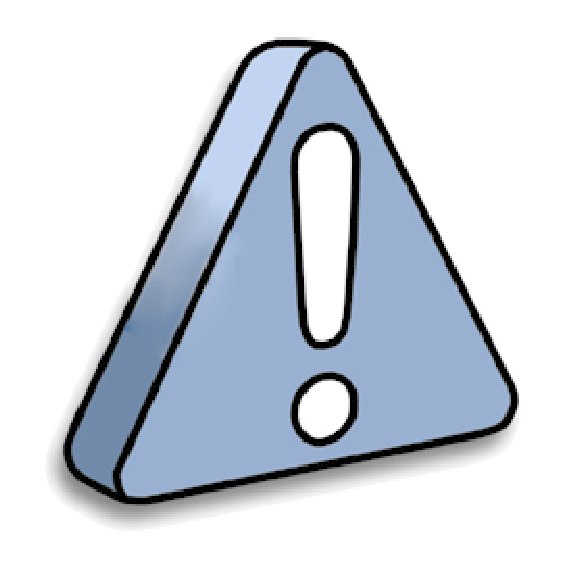
\includegraphics[width=1.5cm]{image/warning}};
  }
\vspace*{20pt}}
%
%%%%%%%%%%%%%%%%%%%%%%%%%%%%%%%%%%%%%%%%
%
%%%%%%%%%%%%%%%%%%%%%%%%%%%%%%%%%%%%%%%%%%%%%%%%
\newtcolorbox{piensa}{
common,
interior code={
  \filldraw[ultra thick,densely dashed,fill=boxbg,draw=black,rounded corners=10pt] (interior.north west) rectangle (interior.south east);
  \node at  ([xshift=-30pt,yshift=10pt]interior.north east) {
\includegraphics[width=1.5cm]{image/tipp}};
  }
\vspace*{20pt}}
%%%%%%%%%%%%%%%%%%%%%%%%%%%%%%%%%%%%%%%%%%%%%%%%%%
\newtcolorbox{resumen}{
common,
interior code={
  \filldraw[ultra thick,densely dashed,fill=boxbg,draw=black,rounded corners=10pt] (interior.north west) rectangle (interior.south east);
  \node at  ([xshift=-30pt,yshift=8pt]interior.north east) {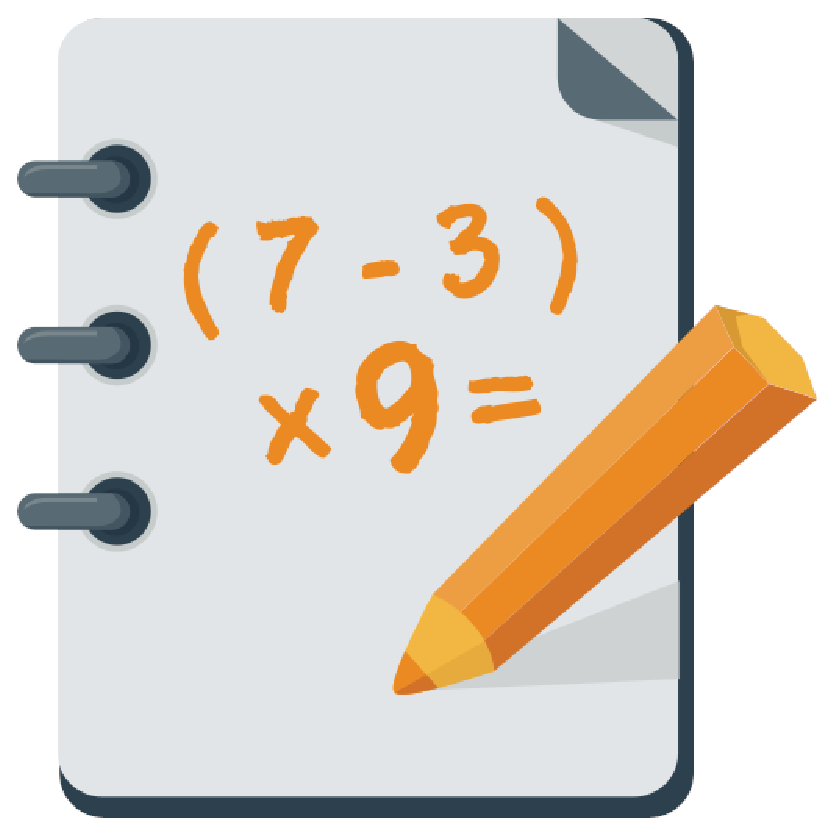
\includegraphics[angle=-30,width=1.5cm]{image/resumen}};
  }
\vspace*{20pt}}
%%%%%%%%%%%%%%%%%%%%%%%%%%%%%%%%%%%%%%%%%%%%%%%%%%%%%%%%%%%%%%%%%%%%%%%
%%%%%%%%%%%%%%%%%%%%%%%%%%%%%%%%%%%%notas para recordar algo%%%%%%%%%%%%%%
\definecolor{paper}{RGB}{239,227,157}
\usetikzlibrary{decorations.pathmorphing}
\newenvironment{notax}[1]{
\begin{tikzpicture}[pencildraw/.style={ %
    decorate,
    decoration={random steps,segment length=2pt,amplitude=1pt}
    } %
]
\node[
preaction={fill=black,opacity=.5,transform canvas={xshift=1mm,yshift=-1mm}},
pencildraw,draw,fill=paper,text width=.8\textwidth,inner sep=5mm] 
{#1};
\end{tikzpicture}
}{\vskip 20pt}
%%%%%%%%%%%%%%%%%%%%%%%%%%%%%%%%%%%%%%%%%%%%%%%%%%%%
\usetikzlibrary{arrows,shadows} 
\newtcolorbox{nota}{%
    enhanced jigsaw, breakable, % allow page breaks
    frame hidden, % hide the default frame
    overlay={%
        \draw [
            fill=ptcbackground, % fill paper
            draw=yellow!20!white, % boundary colour
            decorate, % decoration
            decoration={random steps,segment length=2pt,amplitude=1pt},
            drop shadow, % shadow
        ]
        % top line
        (frame.north west)--(frame.north east)--
        % right line
        (frame.north east)--(frame.south east)--
        % bottom line
        (frame.south east)--(frame.south west)--
        % left line
        (frame.south west)--(frame.north west);
    },
    % paragraph skips obeyed within tcolorbox
    parbox=false,
}
%%%%%%%%%%%%%%%%%%%%%%%%%%%%%%%%%%%%%%%%%%%%%%%%%%%%%%%
%%%%%%%%%%%%%%%%%%%%%%%%%%%%%%%%%%%%%%%%%%%%%%%%%%%
%
\newcounter{praproblem}[chapter]
\renewcommand\thepraproblem{\thesection.\arabic{praproblem}} 
\newtcolorbox{praproblem}{
  before=\bigskip\centering,
    after=\bigskip,
  breakable,
  enhanced,
  colback=white,
  boxrule=0pt,
  arc=0pt,
  outer arc=0pt,
  fontupper=\small,
  title=Problemas para practicar~\thepraproblem,
  fonttitle=\bfseries\sffamily\large\strut,
  coltitle=problemblue,
  colbacktitle=problemblue,
  title style={
    left color=orange!60,
    right color=white,
    middle color=white
  },
  overlay={
    \draw[line width=1.5pt,problemblue] (title.north west) -- (title.north east);
    \draw[line width=1.5pt,problemblue] (frame.south west) -- (frame.south east);
  }
}
\BeforeBeginEnvironment{praproblem}{\refstepcounter{praproblem}}
%
%%%%%%%%%%5
%
\newenvironment{tproblem}[1]{
     
     \begin{praproblem}
     \begin{multicols}{2}
     #1
     \end{multicols}
     }{\end{praproblem}}
%
%%%%%%%%%%%%%%%%%%%%%%%%%%%%%%%%%%%%%%%%%%
%%%%%%%%%%%%%%%%%%%%%%%%%%%%%%%%%%%%%%%%%%%%%%%%%%%%%%
%
\newtcolorbox[auto counter,number within=section]{desafio}{
  breakable,
  enhanced,
  colback=white,
  boxrule=0pt,
  arc=0pt,
  outer arc=0pt,
  title=\textcolor{white}{Problemas desafiantes:~\thetcbcounter,}
  fonttitle=\bfseries\sffamily\large\strut,
  coltitle=problemblue,
  colbacktitle=problemblue,
%  title style={
%  %exercisebgblue
%  interior style={fill=idiomsgreen}
%  },
  overlay={
    \draw[line width=1.5pt,problemblue] (frame.south west) -- (frame.south east);
  }
}

%
%%%%%
%%%%%%%%%%%%%%%%%%%%%%%%%%%%%%%%%%%%%%%%%%%%%%%%%%%%%%%%%%%%%%%%%%%%%%%%%%%%%%%%%%%%%
%%%%%%%%%%%%%%%%%%%%%%%%%%%% problemas %%%%%%%%%%%%%%%%%%%%%%%%%%%%%%%%%%%
\newcommand{\inline}{\refstepcounter{equation}~~\mbox{\color{blue!50!black}(\theequation)}}%enumera eq inline
%%%%%%%%%%%%%%%%%%%%%%% cambiar margenes %%%%%%%%%%%%%%%%%%%%%%%%

\newcommand{\problemas}[1]
{
\section{Ejercicios propuestos}
\small
\begin{adjustwidth}{-1cm}{-4cm} 
%\begin{multicols}{2}
 \noindent #1
%\end{multicols}
{\setlength{\parindent}{0mm}\color{blue!50!black}\rule{\linewidth}{1mm}}
\end{adjustwidth}
}
%%%%%%%%%%%%%%%%%%%%%%%%%%%%%%%%%%%%%%%%%%%%%%%%%%%%%%%%%%%%%%%%%%%%%%%%%%%%
%%%%%%%%%%%%%%%%%%%%%%%%solucion%%%%%%%%%%%%%%%%%%
\newcounter{solucion}[chapter]
%\renewcommand\theexample{\thesection.\arabic{example}}

\tcbset{solucionbox/.style={%
 title={Soluci\'on},
 breakable,
 leftrule=0pt,
 arc=0pt,
 colback=white,
 colframe=titlebgdark,
 enhanced,
 colbacktitle=white,
 coltitle=blue!50!black,
 titlerule=0pt,
 enlarge left by=-4mm,
 width=\linewidth+4mm,
 enlarge top by=2pt,
 overlay unbroken={%
 \draw[titlebgdark,line width=2pt] (frame.north west)++(0,0.25mm) --++(4cm,0pt) ;
                      \draw[white,line width=10mm] (frame.south west) --++(0cm,0pt) node (P) {};
                      \fill[titlebgdark] (P) rectangle ++(6pt,6pt) ;
                      },%
                      %%%%%%%%%%%%%%%
 overlay first={
 \draw[titlebgdark,line width=2pt] (frame.north west)++(0,1pt) --++(4cm,0pt);
 },%
                  %%%%%%%%%%%%%%%%%%%%%%%5
 overlay last={
 \draw[white,line width=10mm] (frame.south west) --++(8cm,0pt) node (P) {};
                       \fill[titlebgdark] (P) rectangle ++(6pt,6pt) ;},%
 }%
}

\newenvironment{solucionn}{%
  \tcolorbox[solucionbox]}%
 {\endtcolorbox}
 %%%%%%%%%%%%%%%%%%%%%%%%%%%%%%%%%%%%%%%%%%%%%%%%%%%%%%%%%%%%%%%%%%%%%%%%%%%%%%%%%%%%%%%%%%%%%%%%
 %%%%%%%%%%%%%%%%%%%%%%%%prueba%%%%%%%%%%%%%%%%%%
\newcounter{prueba}[chapter]
%\renewcommand\theexample{\thesection.\arabic{example}}

\tcbset{pruebabox/.style={%
 title={Prueba},
 breakable,
 leftrule=0pt,
 arc=0pt,
 colback=white,
 colframe=cyan,
 enhanced,
 colbacktitle=white,
 coltitle=cyan,
 titlerule=0pt,
 enlarge left by=-4mm,
 width=\linewidth+4mm,
 enlarge top by=2pt,
 overlay unbroken={\draw[cyan,line width=2pt] (frame.north west)++(0,0.25mm) --++(4cm,0pt);
                      \draw[white,line width=10mm] (frame.south west) --++(8cm,0pt) node (P) {};
                      \fill[cyan] (P) rectangle ++(6pt,6pt) ;},%
 overlay first={\draw[cyan,line width=2pt] (frame.north west)++(0,1pt) --++(4cm,0pt);},%
 overlay last={\draw[white,line width=10mm] (frame.south west) --++(8cm,0pt) node (P) {};
                       \fill[cyan] (P) rectangle ++(6pt,6pt) ;},%
 }%
}

\newenvironment{prueba}{%
  \tcolorbox[pruebabox]}%
 {\hfill \textcolor{ptctitle}{$\blacksquare$}(q.e.d)\endtcolorbox}
 %%%%%%%%%%%%%%%%%%%%%%%%%%%%%%%%%%%%%%%%%%%%%%%%%%%%%%%%%%%%%%%%%%%%%%%%%%%%%%%%%%%%%%%%%%%%%%%%
 \tcbset{demsbox/.style={%
 title={\bf Demostraci\'on:},
 breakable,
 leftrule=0pt,
 arc=0pt,
 colback=white,
 colframe=red!50!black,
 enhanced,
 colbacktitle=white,
 coltitle=red!50!black,
 titlerule=0pt,
 enlarge left by=-4mm,
 width=\linewidth+4mm,
 enlarge top by=2pt,
 overlay unbroken={\draw[red!50!black,line width=2pt] (frame.north west)++(0,0.25mm) --++(4cm,0pt);
                      \draw[white,line width=10mm] (frame.south west) --++(8cm,0pt) node (P) {};
                      \fill[red!50!black] (P) rectangle ++(6pt,6pt) ;},%
 overlay first={\draw[red!50!black,line width=2pt] (frame.north west)++(0,1pt) --++(4cm,0pt);},%
 overlay last={\draw[white,line width=10mm] (frame.south west) --++(8cm,0pt) node (P) {};
                       \fill[red!50!black] (P) rectangle ++(6pt,6pt) ;},%
 }%
}

\newenvironment{dems}{%
  \tcolorbox[demsbox]}%
 {\hfill \textcolor{ptctitle}{$\blacksquare$}(q.e.d)\endtcolorbox}
 %
 %%%%%%%%%%%%%%%%%%%%%%%%%%%%%%%%%%%%%%%%%%%%%%%%%%%%%%%%%%%%%%%%%%%%%%%%\\
 \newenvironment{solver}{\hspace*{-30pt}
    \colorbox{blue!50!black}{%
    \parbox[c][16pt][c]{50pt}{%
    \centering\textcolor{white}{\SectionFont\rmfamily Soluci\'on}}}
    \color{blue!50!black}{\rule{\dimexpr\textwidth-5pt-2\fboxsep\relax}{2pt}}\\[10pt]
       \color{black}
       }{\\[10pt] \color{blue!50!black}{\rule{\dimexpr \textwidth+30pt\relax}{2pt}}\\[20pt]}
      %%%%%%%%%%%%%%%%%%%%%%%%%%%%%%%%%%%%%%%%%%%%%%%%%%%%%%%%%%%%%%%%%%%%%%%%%%%%%
      % normal box
\newcommand{\sqboxs}{1.2ex}% the square size
\newcommand{\sqboxf}{0.6pt}% the border in \sqboxEmpty
\newcommand{\sqbox}[1]{\textcolor{#1}{\rule{\sqboxs}{\sqboxs}}}
% empty box
\newcommand{\sqboxEmpty}[1]{%
  \begingroup
  \setlength{\fboxrule}{\sqboxf}%
  \setlength{\fboxsep}{-\fboxrule}%
  \textcolor{#1}{\fbox{\rule{0pt}{\sqboxs}\rule{\sqboxs}{0pt}}}%
  \endgroup
}

      \newenvironment{probar}{
      \hspace*{-30pt}\colorbox{blue!50!black}{%
    \parbox[c][16pt][c]{80pt}{%
      \centering\textcolor{white}{\SectionFont\rmfamily Demostraci\'on}}}
      \vspace{-1.2\baselineskip}
       \color{blue!50!black}{\rule{\dimexpr\textwidth-5pt-6\fboxsep\relax}{2pt}}
        \\[10pt]     
       \noindent \color{black}\\[10pt]
      }{ \hfill \sqboxEmpty{red!50!black}            
       \color{blue!50!black}{\rule{\dimexpr \textwidth+30pt\relax}{2pt}}\\[20pt]}
       \newcommand{\linea}{{\setlength{\parindent}{0mm}\color{blue!50!black}\rule{\linewidth}{1mm}}}
